% !TeX root = ../thuthesis-example.tex

\chapter{论文工作总体日程安排}

为确保本文的高效进行,本文制定了以下日程安排(图\ref{fig:schedual}),涵盖了论文的各个关键阶段:
\begin{figure}
  \centering
  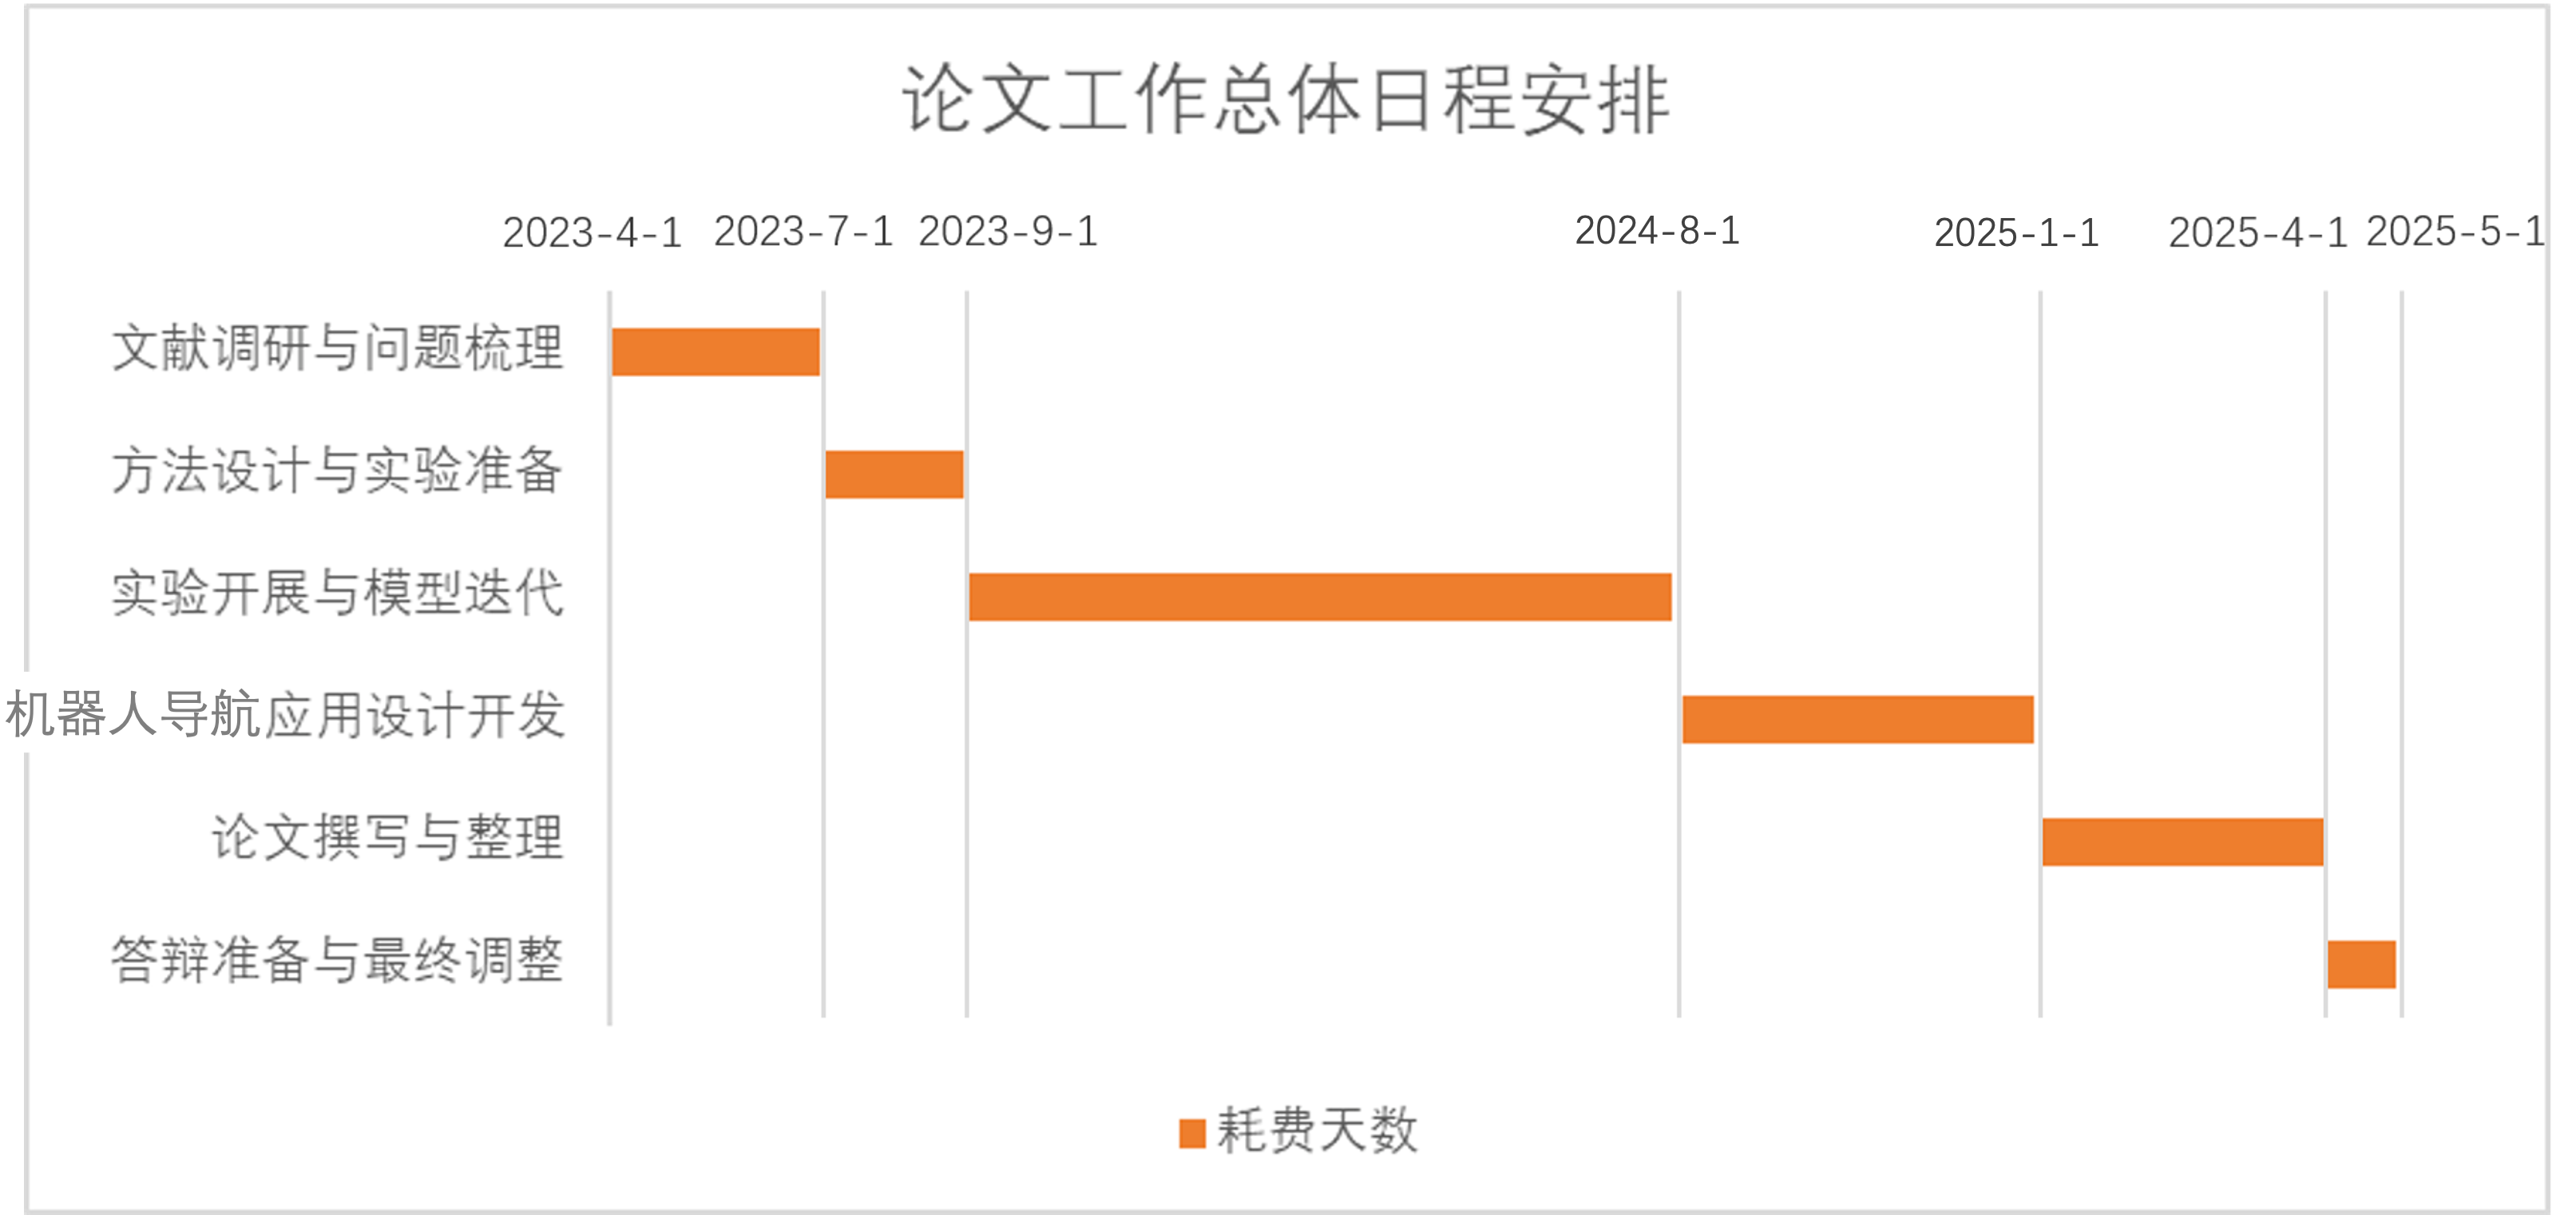
\includegraphics[width=0.85\linewidth]{schedual_new.png}
  % \caption*{}
  \caption{论文工作总体日程安排}
  \label{fig:schedual}
\end{figure}

第一阶段:文献调研与问题梳理(90天)。
深入研究关于动态手势识别、多模态算法以及手势识别应用的相关文献。
总结已有研究的优缺点,并确定本文的定位和问题。

第二阶段:方法设计与实验准备(60天)。
设计手势识别的基本框架与网络结构,深入学习相关深度学习模型和相关算法。
搭建实验环境,准备数据集,确保模型构建的基础工作完成。

第三阶段:实验开展与模型迭代(330天)。
开始初步实验,对框架的可行性进行初步验证。
根据实验结果不断调整框架,优化模型结构,评估模型性能。完善手势识别算法的设计,确保模型能够在实际场景中有效运行。

第四阶段:机器人手势控制应用设计开发(150天)。
详细设计基于所提出手势识别算法的机器人导航控制系统,构建开发机器人手势控制应用,包括离线测试和实际交互控制。

第五阶段:论文撰写与整理(90天)。
撰写论文初稿,%总结实验结果并进行数据分析,设计图表和表格。
逐步完善论文,确保逻辑严密,语言流畅。
进行论文的初步修改和审阅。

第六阶段:答辩准备与最终调整(30天)。
准备论文答辩的相关材料,对论文进行最后的审定和修订,进行论文答辩。

目前研究已经按计划完成前三阶段:文献调研、方法设计与实验,正在开展第四、第五阶段应用开发与论文撰写的工作,预期可按时顺利完成。




